\documentclass[11pt, letterpaper, titlepage]{article}
\usepackage[utf8]{inputenc}
\usepackage[export]{adjustbox}
\usepackage{geometry}
 \geometry{
 a4paper,
 total={168mm,257mm},
 left=20mm,
 top=15mm,
 includefoot,includehead
 }
\usepackage[backend=biber, style=authoryear, giveninits=true, maxbibnames=25, uniquename=init, maxcitenames=2, hyperref=true, dashed=false]{biblatex}			% Benutze Biber/BibLaTeX zum Zitieren
\addbibresource{main.bib}
\usepackage{caption}
\usepackage{subcaption}
\usepackage{graphicx}
\usepackage{svg}
\usepackage{placeins}
\usepackage[hidelinks]{hyperref}
\usepackage{amsmath}
\usepackage[headsepline]{scrlayer-scrpage}
\usepackage{acronym}

\clearpairofpagestyles %Seitenzahl nicht in der Kopfzeile

\title{MeetEU Project - Team Heidelberg - Team 1 -- \\ Identification and Enhancement of novel Sars-CoV-2 NSP13 Helicase Inhibitors}
\author{Linda Blaier, Paul Brunner, Selina Ernst, Valerie Segatz, and Chlo\'{e} Weiler}
\date{February 2024}

\begin{document}

\maketitle

\ihead{\headmark}
\automark{section}  %Kopfzeile gleich dem Sektiontitel
\cfoot{\pagemark}   %\ofood Seitenzahl rechts

\section{Workflow}

\begin{figure}[h]
  \centering
  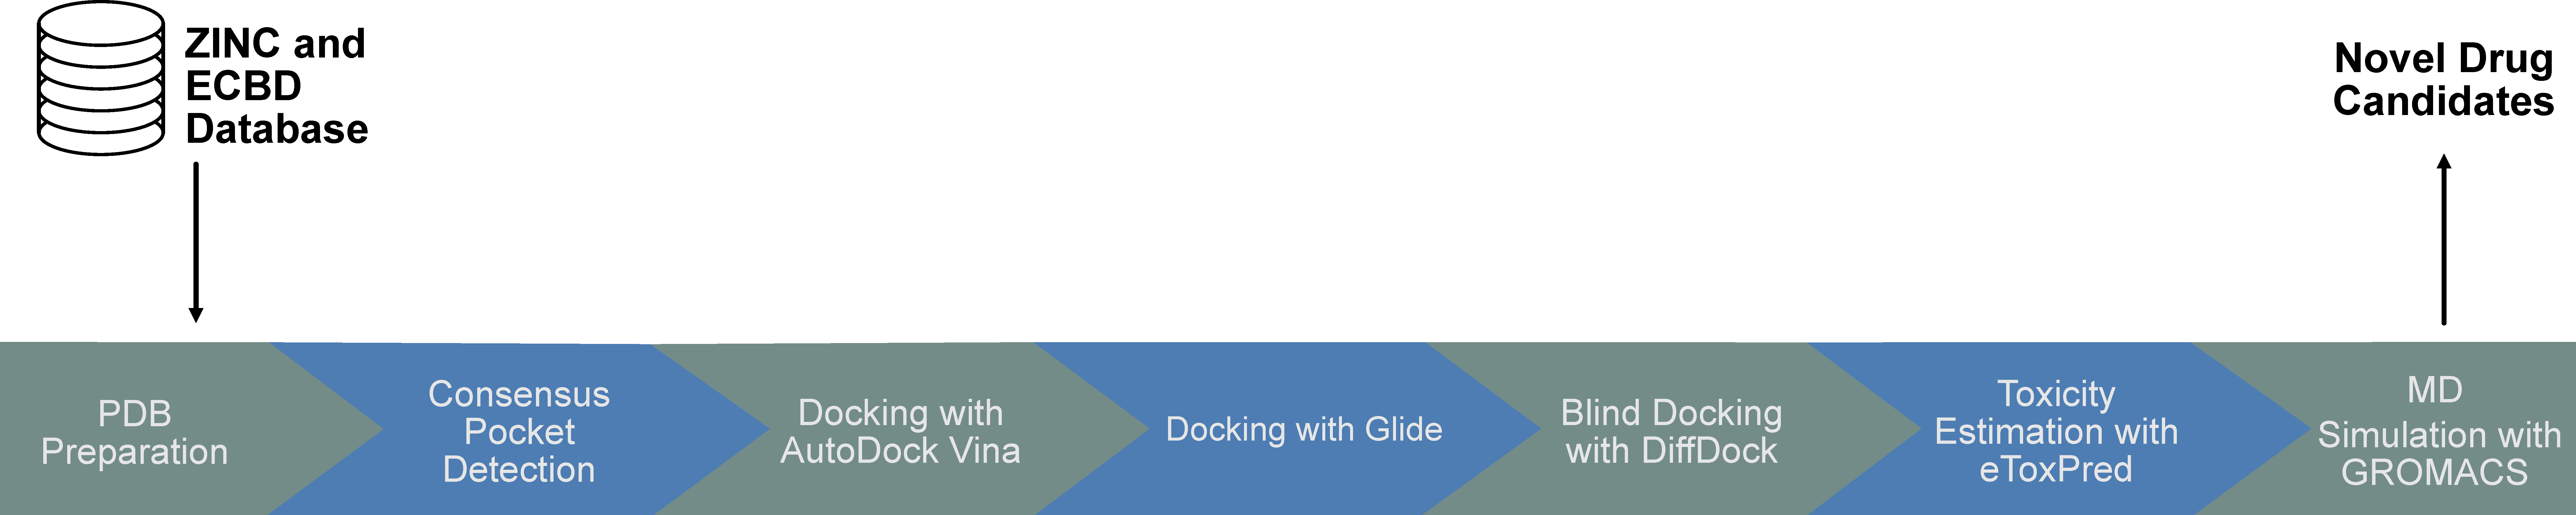
\includegraphics[width=\textwidth]{Workflow_MeetEU.pdf}
  \caption*{\textbf{Proposed workflow for the discovery of NSP13 helicase inhibitors.}Following }
  \label{workflow}
\end{figure}

\setcounter{figure}{0}
\renewcommand{\thefigure}{\arabic{figure}}


\section{Material and Methods}
\subsection{Datasets from ZINC20 and ECBD}
A total of 1616 \ac{FDA}-approved drugs were downloaded in \textit{.sdf} format from the ZINC database \cite{Irwin.2020}. Additionally, 5016 files were retrieved, downloading the pilot library from the ECBD database.

\subsection{Receptor and Ligand Preparation}
\subsection{Consensus binding site detection}
\subsection{Molecular Docking}
\subsection{Estimation of Toxicity and Synthetic Accessibility}
\subsection{Validation of the binding-site for the Top100 scorer}
\subsection{Molecular Dynamics Simulation}

\section{Results}


\FloatBarrier

\section{Discussion and Outlook}



\pagebreak
\FloatBarrier
\renewcommand{\bibname}{References}  % damit Literatuverzeicnis mit "References" betitelt
\printbibliography



\end{document}
